% ------------------------------------------------------------------------------
% TYPO3 Version 11.2 - What's New (English Version)
%
% @author	Michael Schams <schams.net>
% @license	Creative Commons BY-NC-SA 3.0
% @link		https://typo3.org/help/documentation/whats-new/
% @language	English
% ------------------------------------------------------------------------------
% Feature | 93794 | Override TCA description with TSconfig

\begin{frame}[fragile]
	\frametitle{Changes for Integrators and Developers}
	\framesubtitle{TCA Description}

	\begin{itemize}
		\item Since TYPO3 v9, every TCA field can have a description next to
			its label\newline
			For example:
	\end{itemize}
	\begin{figure}
		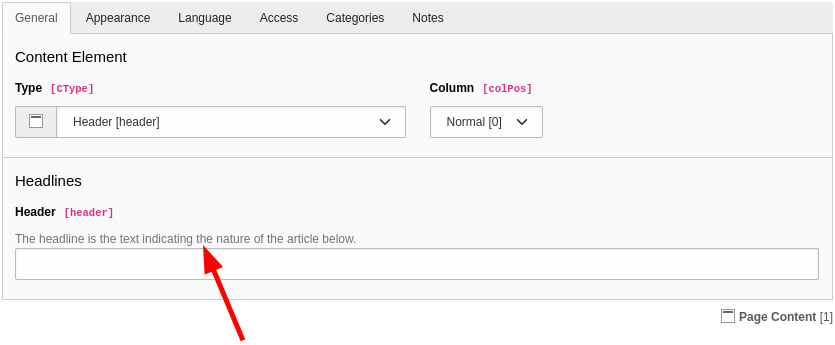
\includegraphics[width=0.70\linewidth]{ChangesForIntegratorsAndDevelopers/11.2/1617959943-TableConfigurationArrayDescription}
	\end{figure}
	\vspace{-0.4cm}
	\begin{itemize}
		\item Integrators can now overwrite the description by using Page TSconfig
	\end{itemize}
\end{frame}

% ------------------------------------------------------------------------------

\begin{frame}[fragile]
	\frametitle{Changes for Integrators and Developers}
	\framesubtitle{TCA Description}

	\lstset{basicstyle=\fontsize{8}{10}\ttfamily}

	\begin{itemize}
		\item This option can also be used to set a description for a field
			that does not feature a TCA description yet
	\end{itemize}

	\begin{itemize}
		\item Example 1 - set/overwrite a description:
\begin{lstlisting}
TCEFORM.<table>.<field>.description = <text>
TCEFORM.tt_content.header.description = The headline is the text...
\end{lstlisting}
		\item Example 2 - on a per record type basis:
\begin{lstlisting}
TCEFORM.<table>.<field>.types.<type>.description = Description for <type>
\end{lstlisting}
		\item Example 3 - referring to a language file:
\begin{lstlisting}
TCEFORM.tt_content.header.description = LLL:EXT:my_ext/Resources/Private/Language/locallang.xlf:description
\end{lstlisting}

	\end{itemize}

\end{frame}

% ------------------------------------------------------------------------------
